\documentclass[a4paper, 10pt]{article}
\usepackage{palatino}
\usepackage[a4paper]{geometry}
\usepackage[UKenglish]{babel}
\usepackage[utf8]{inputenc}
\usepackage{afterpage}
\usepackage{fancyhdr}
\usepackage{amsmath}
\usepackage{amstext}
\usepackage{amssymb}
\usepackage{physics}
\usepackage{derivative}
\usepackage{longtable}
\usepackage{tabularx}
\usepackage{dcolumn}
\usepackage{graphicx}
\usepackage{enumerate}
\usepackage{multicol}
\usepackage{pdfpages}
\usepackage{lastpage}
\usepackage{siunitx}
\usepackage{listings}
\usepackage{tikz}
\usepackage{xspace}
\usepackage{caption} 

\AtBeginDocument{\RenewCommandCopy\qty\SI}
\sloppy

\geometry{margin=25mm, top=20mm, bottom=20mm}
\captionsetup{format=plain,indention=0mm, font=small, labelfont=bf, labelsep=period}

\newcommand{\logo}{\begin{figure}[!t] \vspace*{-10mm} \hspace*{-10mm}

\includegraphics[height=23mm]{../defs/usn-logo-en.pdf} \end{figure}}

\newcommand{\labfoot}[1]{\fancyhf[FC]{ \textit{TSE2280, Lab exercise  #1, spring 2024} } }

\newcommand{\regneovinglosningfoot}[1]{\fancyhf[FC]{TSE2280 Regneøving #1 - Løsning }}
\newcommand{\regneovingtitle}[1]{\section*{TSE2280, våren 2024. \qquad Regneøving #1 }}
\newcommand{\regneovinglosningtitle}[1]{\section*{TSE2280, Måleteknikk og signalbehandling \\Løsning regneøving #1 }}

\newcommand{\Fig}[1]{Fig.~\ref{fig:#1}}
\newcommand{\tableref}[1]{Table~\ref{tab:#1}}

\newcommand{\ed}[1]{\ensuremath{\cdot10^{#1}}}
\renewcommand{\deg}{\ensuremath{^\circ}}
\newcommand{\omegahat}{\hat \omega}

\newcommand{\zm}[1]{ z^{-{#1} } }

\newcommand{\ew}[1]{e^{{#1}j \omegahat }}
\newcommand{\ewn}[2]{e^{{#1}j{#2}} }
\newcommand{\Hw}[1]{H\left( e^{{#1}j \omegahat} \right)}
\newcommand{\Hwn}[2]{H \left( e^{{#1}j {#2}} \right)}

\newcounter{problem}
\newcommand{\problem}[1]{\stepcounter{problem}\section*{Problem \arabic{problem}. {#1}}} 

\newcommand{\subproblem}{\begin{enumerate}[a)]}
\newcommand{\subproblemend}{\end{enumerate}}

%=== FIGURE DEFINITIONS ============
\newenvironment{stdfig}{\begin{figure}[!b]\begin{center}}{\end{center}\end{figure}}
\newcommand{\stdgraphics}[1]{\begin{center}\includegraphics[width=0.95\textwidth]{#1}\end{center}}
\newcommand{\scaledgraphics}[2]{\begin{center}\includegraphics[width={#1}\textwidth]{#2}\end{center}}
\newcommand{\includescanFB}[1]{\begin{center}\includegraphics[width=0.90\textwidth]{#1}\end{center}}
\newcommand{\includescanMcC}[1]{\includegraphics[width=0.80\textwidth]{#1}}
\newcommand{\includedrawing}[1]{\includegraphics[scale=0.65]{#1}}
\newcommand{\Matlabfigure}[1]{\includegraphics[scale=0.80]{#1}}

\newcommand{\losning}[1]{\includegraphics[width=0.85\textwidth]{./losninger/#1}}
\newcommand{\losningfig}[1]{\includegraphics[width=0.85\textwidth]{./figs/#1}}
\newcommand{\losningfigfull}[1]{\includegraphics[width=0.99\textwidth]{./figs/#1}}
\newcommand{\losningfighalf}[1]{\includegraphics[width=0.49\textwidth]{./figs/#1}}
\newcommand{\losningfigreduced}[1]{\includegraphics[width=0.49\textwidth]{./figs/#1}}

%=== REFERENCING ===========================================
\newcommand{\Eq}[1]{(\ref{eq:#1})}

% Headers and footers
\pagestyle{fancy}
\renewcommand{\headrulewidth}{0pt}
\renewcommand{\footrulewidth}{0pt}

\fancyhf{} 
\fancyhf[FL]{\textit{\small LH, \today} }
\fancyhf[FR]{Page \thepage\ of \pageref{LastPage}} 


% Style for program listing
\definecolor{codegreen}{rgb}{0, 0.5, 0}
\definecolor{codegray}{rgb}{0.5, 0.5, 0.5}
\definecolor{codepurple}{rgb}{0.58, 0, 0.82}
\definecolor{backcolour}{rgb}{0.98, 0.98, 0.95}

\lstdefinestyle{pythonstyle}{
	language=python,	
	belowcaptionskip=1\baselineskip,
	breaklines=true,
	frame=single,
	numbers=none, 
	breaklines=true,				 
	keepspaces=true,		
	breakatwhitespace=false,		 		 	
	basicstyle=\small\ttfamily,
	keywordstyle=\color{blue},
	stringstyle=\color{codepurple},	
	commentstyle=\color{codegreen},
	identifierstyle=\color{black!95!white},
	backgroundcolor=\color{backcolour},
	tabsize=4,	
	}
\labfoot{2}
\hyphenpenalty=5000
\newcommand{\numpy}{NumPy\xspace}
\newcommand{\matplotlib}{Matplotlib\xspace}
\newcommand{\scipy}{SciPy\xspace}
\newcommand{\cmath}{cmath\xspace}
\newcommand{\jupyterlab}{JupyterLab\xspace}

\begin{document}
\logo

\title{Introduction to Complex Exponentials \\ Direction Finding} 
\author{TSE2280 Signal Processing. Lab 1}
\date{Spring 2025}
\maketitle

\thispagestyle{fancy}	

\section{Introduction}
\suppressfloats[t]
This lab is a modified version of the lab \emph{Lab P-3: Introduction to Complex Exponentials – Direction Finding}\cite{mcclellan_lab_2016} that accompanies the course text-book \emph{DSP First} by McClellan et~al \cite{mcclellan_dsp_2016}. The original lab has been converted from Matlab to Python and some of exercises have been changed. 

The lab demonstrates concepts from Chapters 2 and 3 in the text-book. The intention is to give a better understanding of sinusoidal signals and how they are described by complex amplitude vectors, \emph{phasors}.

The exercise was made for the course \emph{TSE2280 - Measurements and Signal Processing} taught at the University of South-Eastern Norway.

\subsection{Aim}
The first part of this lab gives training in how to create and manipulate sinusoidal signals using complex exponentials in Python. The last part uses this to estimate the direction of a sound source from the phase difference between signals received by two microphones. 
This type of direction estimates is the basis for steering and focusing ultrasound beams with \emph{phased arrays} in sonar and medical ultrasound. The same principle is also used to steer radar beams and in wifi and 5G antennas.

This lab is a computer simulation only, but can be extended to a real situation withou much extra equipment. Record a sound with two microphones using the stereo channels in your sound card, and then test the method on the recorded signal.


\subsection{Software Tools: Python with Spyder and \jupyterlab}
The programs for the lab shall be written in Python using the modules \numpy for representing signals and \matplotlib for plotting graphs. Later exercises will use the signal processing module in \scipy (\texttt{scipy.signal}) but \scipy is not needed in this exercise.

Python's module for complex numbers \cmath can make the code easier to read. But be aware that \cmath handles scalar numbers only. The signals are more conveniently represented by arrays as in \numpy.
The recommended setup of libraries for this exerceise is shown in \tableref{import-libraries}

The recommended Python programming environment for this and the following labs is \emph{Spyder}\cite{raybaut_spyder_2024}, which is included in the \emph{Anaconda}\cite{noauthor_anaconda_2024} package management. However, any Python package management and programming environment should function.

All code files shall be included with the lab report. We recommend collecting everything, code, text and figures, into a single \jupyterlab Notebook\cite{project_jupyter_jupyter_nodate}, but a pdf with separate Python files is also acceptable.


\begin{table}[t!]
\caption{Recommended format for importing the Python modules. \numpy is used to manipulate signals as arrays, \matplotlib to plot results.
The complex math library \cmath can be included to have simpler access to mathematical constants and functions, e.g., $\pi$, the complex exponential, and the square root.}
\label{tab:import-libraries}
\begin{lstlisting}[style=pythonstyle]]
		
import numpy as np
import matplotlib.pyplot as plt
from cmath import pi, exp, sqrt     # For readability, also covered by NumPy
		
\end{lstlisting}
\end{table}


\section{Theory}

\subsection{Sinusoidal Signals and Phasors}
The aim of the first part of this lab is to obtain experience with complex numbers, and using phasors and complex exponentials to represent sinusoidal signals.
Recall from the lectures that a sinusoidal signal $x(t)$ is written as 
\begin{align}
	x(t)&= A cos(\omega t + \phi) = \Re\left\{ A e^{j(\omega t + \phi)} \right\} 
		=  \Re\left\{ X e^{j\omega t} \right\} \quad , &
	X &= A e^{j\phi} 
\end{align}
where $A$ is the amplitude, $\omega = 2\pi f$ is the angular frequency, $f$ is the frequency, and $\phi$ is the phase. $	X = A e^{j\phi} $ is a \emph{phasor} or \emph{complex amplitude} that includes both the amplitude and the phase of the signal.
Analysis of sinusoidal signals like $x(t)$ is in general simpler by manipulating phasors as complex numbers compared to using the amplitude and phase separately.

\subsection{Complex Numbers in Python with \numpy}
Analysis of complex quantities in Python is simple. When using the library \numpy, complex numbers are handled almost exactly as real numbers, i.e.~most of the usual mathematical operators and functions can be used on complex numbers.

\tableref{complex-overview} lists the basic operations in complex numbers in Python using \numpy. Note that all function calls in this table are prefixed by \verb|np| due to the way \numpy was imported, see \tableref{import-libraries}. Note also that a complex number in Python has three public members, \verb|real|, \verb|imag|, and \verb|conjugate()|.

\begin{table}[t!]
	\caption{Overview of basic complex number operations in Python. Details are found in the documentation for \numpy.
	The function calls are prefixed by \texttt{np} in accordance with how \numpy was imported, see \tableref{import-libraries}. }
	\label{tab:complex-overview}
\begin{tabular}{llll}
	%\hline
	Command					& Member & Description					& Mathematical notation \\
	\hline
	\\
	\verb|z = complex(2,3)| & & Creates a complex number.	& $z= x + jy = 2 + 3j$. \\
	\verb|z = 2 + 3j| 		& & Same as above \\
	\verb|1j| 				& &	Imaginary unit, $i$ or $j$.		& $i = j = \sqrt{-1} $	\\ 
	\\
	\verb|np.conj(z)|  	& \verb|z.conjugate()| & Complex conjugate.	& $z^*= x -jy $ \\
	\verb|np.abs(z)|	&			& Absolute value.	&  $|z|= \sqrt{x^2 + y^2}$ \\
	\verb|np.angle(z)| 	&			& Phase in radians.	& $\angle z  $ 	\\
	\verb|np.real(z)| 	& \verb|z.real|	&	Real part.			& $\Re\{z\} = x  $  \\
	\verb|np.imag(z)| 	& \verb|z.imag|	&	Imaginary part.		& $\Im\{z\} = y $	\\ 
	\verb|np.exp(1j*theta)|	& 		&Complex exponential. 	& $e^{j\theta} = cos\theta + j\sin\theta$ \\
	\\
	\hline 
\end{tabular}
\end{table}

\subsection{Adding Sinusiods using Complex Exponentials}
Sinusoidal signals are most conveniently handled using complex exponentials. The theory behind this is given in Chapter 2 in the textbook and was presented in the lectures. It is briefly summarised here.

Look at a signal that is the sum of sinusoids that all have the same $f_0$, while the amplitude $A_k$ and phase $\phi_k$ of the individual signals can be different, 
\begin{align}
	x_s(t)= \sum_{k=1}^{N} A_k \cos(2\pi f_0 t + \phi_k)   \:.
\end{align}
The resulting summed signal can be found by summing the complex exponentials and then taking the real part. This is called \emph{phasor summation} and is  easier than using trigonometric identities, 
\begin{align}
	x_s(t)= \Re\left\{ \sum_{k=1}^{N}  A_k e^{j\phi_k} e^{j2\pi f_0 t } \right\}  
			= \Re\left\{ \sum_{k=1}^{N}  X_k  e^{j2\pi f_0 t } \right\}  \:.
	\label{eq:phasorsum}
\end{align}
The \emph{complex amplitude }or \emph{phasor} $X_k$ is defined as 
\begin{align}
	X_k &= A_k e^{j\phi_k} \:.
\end{align}
The factor $ e^{j2\pi f_0 t}$ in \Eq{phasorsum} is equal for all the individual signals, i.e., independent of $k$, so the amplitude $A_k$ and phase $\phi_k$ of the summed signal $x_s(t)$ can be found by summing the complex amplitudes, 
\begin{align}
	x_s(t)&= \Re \left\{ X_s e^{j\omega t } \right\} = A_s \cos(2\pi f_0 t + \phi_s)  \:,
	 &  X_s&= \sum_{k=1}^{N} X_k = A_s e^{j\phi_k}  \:.
\end{align}
The resulting signal will have the same frequency $f_0$ and period $T_0=1/f_0$ as the original signals. 

\subsection{Harmonics and Periodic signals}
Consider now a signal $x_h(t)$ where the frequencies $f_k$ of the individual cosine-waves are different, but are integer multiples of a fundamental frequency $f_0$, 
\begin{align}
	f_k& = k f_0 \quad , & k&= 0,1,2, \ldots \:.
\end{align}
The individual signals $\cos(2\pi k f_0 t +\phi_k)$ are called \emph{harmonics} and the summed signal $x_h(t)$ can be written as
\begin{align}
	x_h(t)= \sum_{k=1}^{N}  A_k \cos(2\pi k f_0 t +j\phi_k)
	= \Re\left\{ \sum_{k=1}^{N}  X_k  e^{j2\pi k f_0 t } \right\}  \:.
	\label{eq:harmonicsum}
\end{align}
The periods $T_k$ of the individual waves are 
\begin{align}
	T_k &= T_0/k
\end{align}
After the period $T_0=k T_k$ of the fundamental frequency, the individual signals have repeated themselves $k$. Hence, all he frequency components will also be periodic with period $T_0$, and the resulting signal $x_h(t)$ will be periodic with period given by the fundamental frequency $f_0$ as $T_0=1/f_0$.

\section{Programming Tips}

\subsection{Complex Numbers and Phasors}
The Python file \verb|zplot.py| contains functions to plot complex numbers as phasors, add them, and show the resulting phasor plots and sinusoids. 
The the description for the function \verb|phasor()| in  \verb|zplot|  is shown in \tableref{zplot}.

\begin{table}[h!]
\caption{Function \texttt{phasor()} to show complex numbers as phasors in the complex plane (Argand-diagrams). The functions are found in the file \texttt{zplot.py} included for this lab. }
\label{tab:zplot}
\begin{lstlisting}[style=pythonstyle]]

def phasor(zk,
		   labels=[],
		   include_sum=False,
		   include_signal=False,
		   frequency=1):
	"""Show complex amplitudes and resulting signals.

	Parameters
	----------
	zk : Complex or list of complex
		Complex numbers to show
	
	labels=[] : List of strings, optional
		List of labels to mark phasors
	
	include_sum=False : Boolean, optional
		Show the sum of all numbers as a phasor
	
	include_signal=False : Boolean, optional
		Include a plot of signals as function of time
	
	frequency=1 : Float, optional
		Frequency used to plot the signals
	
	Returns
	-------
	ax : List of Matplotlib Axes
		Handle to axes containing the plots
	"""
	
\end{lstlisting}
\end{table}

\subsection{Vectorization}
\numpy module allows mathematical operations to be used on arrays. This is convenient when defining signals such as $x(t)=A \cos(2\pi f t + \phi)$. Here, the amplitude $A$ and phase $\phi$ are scalars, while the time $t$ is a vector spanning the time interval to be investigated. 

Vectors spanning e.g., a time interval are created in \numpy by one of these methods

\begin{enumerate}[1)]
	\item Specifying start, stop and step by the function \texttt{arange}. \\ 
	 A time vector $t$ is  typically defined as 
	 \verb|  t = np.arange(t_start, t_end, dt|), \\
	 where \verb|t_start| is the first point in the time-vector \verb|t|, \verb|t_end| marks the end of \verb|t|, and \verb|dt| is the interval between the time points. Note that the value \verb|t_end| is not included in the time vector, \verb|t| will end on the last point before \verb|t_end|.
	 
	\item Specifying start, stop, and total number of points by the function \texttt{linspace}. \\
	A time vector $t$ is typically defined as \verb| t = np.linspace(t_start, t_end, n_points)|, \\
	where \verb|t_start| is the first point in $t$, \verb|t_end| marks the end of \verb|t|, and \verb|n_points| is number of points in the vector. 
	Note again that the last value \verb|t_end| is not included in the time vector, \verb|t| will end on the last point before \verb|t_end|.

	\item Specifying start, stop, and total number of points by the function \texttt{logspace}. \\ 
	This is the same as \verb|linspace|, but the numbers are evenly spaced on a logarithmic scale, and the start and end points are specified by their logarithms: \verb|start=2| means the first value is \num{e2}=\num{100}.
\end{enumerate}
	


\section{Training Exercises}

\subsection{Complex Numbers}
The purpose of this task is to get used to complex numbers, how to visualize them as phasors, and how to use them in Python.

\subsubsection*{Reporting}	
Collect the answers and code in one notebook in Jupyter Lab and upload this to Canvas.

\subsubsection*{Exercises}	
\begin{enumerate}[1)]
	\item Load the library \verb|zplot| to visualize the results.

	\item Enter the two complex numbers $z_1 = 2e^{j\pi/3}$ and $z_2= -\sqrt{2} + 5j$. 
	
		Use the Python functions or methods to find the real and imaginary part, $\Re\{z\}$ and $\Im\{z\}$, the magnitude $|z|$ and phase $\angle z$ .
	
		Display $z_1$ and $z_2$ and the sum $z_1+z_2$ as phasors with \verb|zplot.phasor|. 		
		The input to \verb|zplot.phasor| is specified as a \verb|list|, this is done by enclosing the numbers in square brackets, e.g., \verb|[z1, z2]|.

	\item Find the complex conjugate $z^*$ and inverse $1/z$ for $z_1$ and $z_2$ and plot them using \verb|zplot|.
	
		Recall what you have learned about complex numbers in math courses. Are the results as expected?
			
	\item Calculate the product $z_1 z_2$ and ratio $z_1/z_2$ and plot them using \verb|zplot|. 
	
		Are these results as expected?

	\item Calculate the products of the conjugates, $z_1 z_1^*$ and $z_2 z_2^*$. 
	
	Plot them in the same diagram as $z_1$ and $z_2$ and explain the result.

	\item Calculate the sums $z_1+z_1^*$ and differences $z_1-z_1^*$ of the conjugates and plot them in the same diagram as $z_1$. Do the same for $z_2$. Explain these results.
		
\end{enumerate}

		
		
\subsection{Python Function to Generate a Sinusoid Signal }

\subsubsection*{Reporting}	
Collect the answers and code in one notebook in Jupyter Lab and upload this to Canvas.

\subsubsection*{Exercises}	

\begin{enumerate}[1)]
	\item Write a function (\verb|def| in Python) that generates a single sinusoid, $x(t)= A \cos(\omega t + \phi)$ from the four input arguments amplitude $A$, frequency $f$, phase $\phi$ and duration. The angular frequency is $\omega=2\pi f$.
	
	The function shall return the sinusoidal signal $x(t)$ and the time vector $t$ where the signal is evaluated.
	
	The function shall generate exactly 32 values of the sinusoid per period. 

	A skeleton of the function with the recommended function call and ducumentation string is listed in \tableref{make-cos}. 

	\item Demonstrate that your function works by plotting the output for the following parameters:
		\begin{align*}
			A&=\num{e4} & f&= \qty{1.5}{MHz} &	\phi&=-\ang{45} & \text{Duration \qty{e-6}{s}}
		\end{align*}		
		Note that the phase must be converted to radians before calculating the result. 
		What is the phase in radians in this case?
		
		Use \matplotlib to plot the results.
				
		Calculate the value of $x(t)$ at $t=0$. Does this agree with the plot?

	\item Calculate the period of the resulting signal and check that this agrees with the plot.
\end{enumerate}

\begin{table}[h!]
	\caption{Skeleton for a function to generate a cosine signal from amplitude, frequency, and phase.
	The first lines are the recommended function call and docstring. The last line specifies that the signal \texttt{x} and time vector \texttt{t} are returned. }
	\label{tab:make-cos}
\begin{lstlisting}[style=pythonstyle]]

def make_cos(A, f0, phase, duration):
	"""Make a cosine-function from specified parameters.
	
	Parameters
	----------
	A : float
		Amplitude
	f0: float
		Frequency [Hz]
	phase: float
		Phase [radians]
	duration: float
		Duration of signal [seconds]
	
	Returns
	-------
	x: 1D array of float
		Cosine-wave
	t: 1D array of float
		Time vector [seconds]
	"""
	
	--- Your code comes here ---
	
	return x, t
		
\end{lstlisting}
\end{table}

\subsection{Python Function to Generate a Sum of Sinusoid Signals}
Signals are often described as a sum of sinusoids with different amplitudes $A_k$, frequencies $f_k$, and phases $\phi_k$.
Hence, it can be convenient to have a function that generates a signal from several cosine-functions, each specified by its amplitude, frequency, and phase.

\subsubsection*{Reporting}	
Collect the answers and code in one notebook in Jupyter Lab and upload this to Canvas.

\subsubsection*{Exercises}	

\begin{enumerate}[1)]
	\item Write a function that generates a signal
	\begin{align}
		x(t)= \sum_{k=1}^{N} A_k \cos(2\pi f_k t + \phi_k) =\sum_{k=1}^{N} X_k e^{j2\pi f_k t}.
	\end{align}
	The input arguments are the complex amplitude $X_k=A_k e^{j\phi}$, frequency $f_k$, sample rate $f_s$ and the signal duration.
	
	The function shall return the summed signal $x(t)$ and the time vector $t$ where the signal is evaluated.
	
	The frequencies $f_k$ and complex amplitudes $X_k$ shall be specified as \numpy arrays, and the function shall accept any number of frequency components. 
	
	Each frequency $f_k$ shall match a complex amplitude $X_k$, so these vectors must have equal length. The resulting function must check for this and shall return an error message if the lengths are different. 
	
	A skeleton of the function with the recommended function call and header is listed in \tableref{summed_cos}. 
		
	\item Demonstrate that your function works by plotting the output for a signal that is the sum of the following components.
	\begin{center}
		\begin{tabular}{ccc}
				&	Frequency	& Complex amplitude	\\
			k	&	$f_k$ [Hz]		& $X_k$  			\\
			\hline
			1	&	\num{0}		& \num{10}				\\
			2	&	\num{100}	& $14e^{-j\pi/3}$		\\
			3	&	\num{250}	& 	$8j$				\\
		\hline
		\end{tabular}
	\end{center}
	Set the sample rate to \qty{10000}{Samples/s}, the duration of the signal to \qty{0.1}{s}, and the start time to \qty{0}{s}. Plot the result with \matplotlib.
	
	\item Measure the period $T_0 $ of the signal from the graph. Compare this to the periods $T_k$ of the individual frequency components $f_k$.
	
	Explain how the period of the summed signal can be calculated from the periods of the individual components.
	
	\item Generate the signal
	\begin{align*}
		x(t) &= \Re{-2e^{j50\pi t} - e^{j50\pi(t-0.02)} +(2-3j)e^{j50\pi t}   } 
	\end{align*}
	over a time range that covers 3 periods. 
	
	Plot the signal $x$ a function of time $t$.
	
	\item The signal above contains frequency that are all equal. In this case, the amplitude and phase can be calculated by summing its complex amplitudes, \emph{phasors}.
	
	Use the function \verb|zplot.phasor| from the first exercise to pot the phasor diagram for this signal.
	
	\verb|zplot.phasor| has optional arguments that can be set to illustrate this better
	
	\begin{tabular}{ll}
		\verb|include_sum = True| & Add the sum of all the phasors to the plot. \\
		\verb|include_signal = True| & Plot the signals corresponding to the phasors. \\
		\verb|frequency = <value>|  & Frequency to use when plotting the signals.
		
	\end{tabular}

\end{enumerate}

\begin{table}[t!]
	\caption{Skeleton for a function to generate signal by summing cosine-functions with different complex amplitudes and frequencies.		
	The first lines are the recommended function call and docstring. The last line specifies that the signal \texttt{x} and time vector \texttt{t} are to be returned. 	
	Note how the start time \texttt{t\_start} is specified as an optional argument with default value \num{0}.
	}
	\label{tab:summed_cos}
	
\begin{lstlisting}[style=pythonstyle]

def make_summed_cos(fk, Xk, fs, duration, t_start=0):
	"""Synthesize a signal as a sum of cosine waves

	Parameters
	----------
	fk: List of floats
		Frequencies [Hz]
	Xk: List of floats
		Complex amplitudes (phasors)
	fs: float
		Sample rate [Samples/second]
	duration: float
		Duration of signal [s]
	t_start=0 : float, optional
		Start time, first point of time-vector [seconds]
	
	fk and Xk must have the same lengths.

	Returns
	-------
	x: 1D array of float
		Signal as the sum of the frequency components
	t: 1D array of float
		Time vector [seconds]
	"""

	--- Your code comes here ---

	return x, t
	
\end{lstlisting}
\end{table}

\section{Lab Exercise: Direction finding}
The text in this exercise is taken from \cite{mcclellan_lab_2016}, with some small modifications.

Why do humans have two ears? One answer is that the brain can process acoustic signals received at the two ears and determine the direction to the source of the acoustic energy. Using sinusoids, we can describe and analyze a simple scenario that explains this direction finding capability in terms of phase differences (or time-delay differences). 

This same principle is used in many other applications including radars that locate and track airplanes, and it gives the basis for phased array transducers used in medical ultrasound and sonar.

\subsection*{Reporting}	
Collect the answers and code in one notebook in Jupyter Lab and upload this to Canvas.

\subsection{Exercises: Direction Finding with Microphones}
Consider a simple measurement system that consists of two microphones that can both hear the same source signal. If the microphones are placed some distance apart, then the sound must travel different paths from the source to the receivers. When the travel paths have different lengths, the two signals will arrive at different times. Thus a comparison of the two received signals will allow us to measure the relative time difference (between peaks), and from that we can calculate the direction. If the source signal is a sinusoid, we can measure the travel time differences by measuring phases.

The scenario is illustrated in \Fig{overview} where a vehicle travelling on the roadway has a siren that is transmitting a very loud sinusoidal waveform whose frequency is $f_s$=\qty{400}{Hz}. The roadway forms the $x$-axis of a coordinate system.

The two receivers (microphones) are located some distance away and are aligned parallel to the roadway. The distance from the road is $y_r$=\qty{100}{m}, and the receiver separation is $d$=\qty{0.4}{m}. The signals at the receivers must be processed to find the angle from Receiver M1 to the vehicle, which is denoted as $\theta$ in Fig. 1.

\begin{stdfig}
	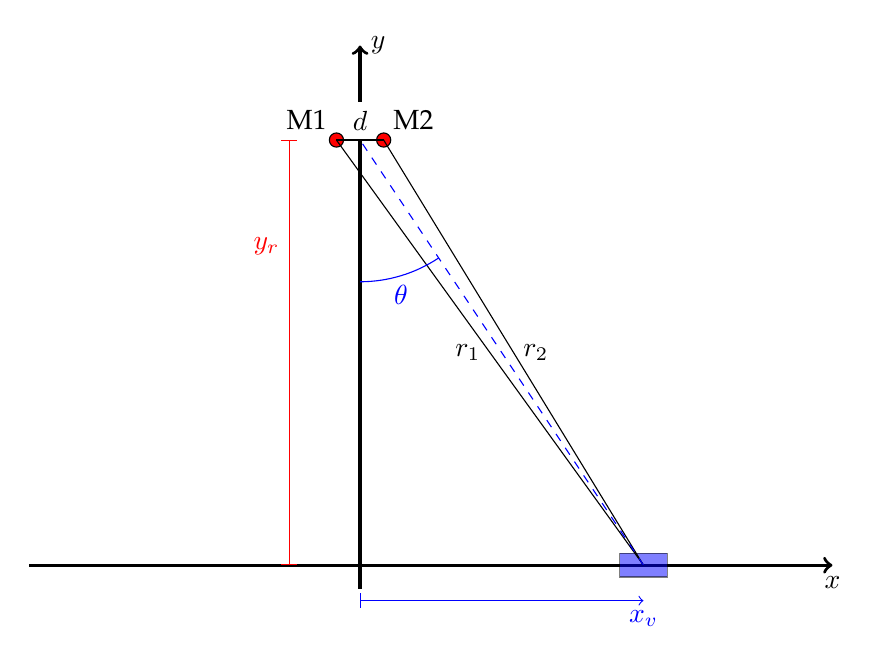
\begin{tikzpicture}[scale=3][>=stealth]

	\def\angle{33.7}
	\def\ymax{2.2}
	\def\xmax{2.0}
	\def\yr{1.8}
	\def\xv{1.2}
	\def\d{0.2}
	\def\sourcesize{0.03}
	
	% Colours
	\colorlet{anglecolor}{blue} 
	\colorlet{roadcolor}{gray!20!black} 
	\colorlet{ycolor}{red} 
	\colorlet{xcolor}{blue}
	
	% Styles  
	\tikzstyle{axisline}=[very thick] 
	
	% Axes and road
	%\filldraw[fill=roadcolor, draw=black, nearly transparent] (-\xmax/2, -0.02) rectangle (\xmax*0.9, +0.02);
	\draw[axisline, ->] (-\xmax*0.7, 0) -- (\xmax, 0)  node[below]{$x$};
	\draw[axisline, ->] (0, -0.1) -- (0, \ymax)  node[right]{$y$};
	\filldraw[fill=xcolor, draw=black, semitransparent] (\xv-0.1, -0.05) rectangle  ++(0.2, 0.1) ;
	
	% Microphones
	\filldraw[fill=ycolor, draw=black] (-\d/2, \yr) coordinate(M1) circle (\sourcesize);
	\filldraw[fill=ycolor, draw=black] (\d/2, \yr) coordinate(M2) circle (\sourcesize);
	\draw[- ] (M1) -- node[above, midway, fill=white!] {$d$} (M2);

	% Sound paths
	\draw[-] (\xv, 0) -- (M1) node[above left]{M1}  node[midway, anchor=east]{$r_1$};
	\draw[-] (\xv, 0) -- (M2) node[above right]{M2} node[midway, anchor=west]{$r_2$};;
	\draw[-, dashed, anglecolor] (\xv, 0) -- (0,\yr);
		
	% Angle
	\draw[draw=anglecolor] (0,\yr)++(0, -0.6)  arc(-90:-90+\angle:0.6) coordinate(ARC) 
		node[midway, below, anglecolor]{$\theta$};

	% Rulers
	\draw[|->, xcolor] (0, -0.15) -- ++(\xv, 0) node[at end, below]{$x_v$};
	\draw[|-|, ycolor] (-0.3, 0) -- ++(0, \yr) node[near end, left]{$y_r$};

\end{tikzpicture}


	\caption{Direction finding using two microphones. A vehicle at position $x_v$ travels along the $x$-axis while emitting a sound with frequency $f_s$=\qty{400}{Hz}. The sound is picked up by two microphones M1 and M2 positioned with spacing $d$=\qty{0.40}{m}. The difference in propagation distance $\Delta r=r_1-r_2$ causes a phase-shift between the signals received by the two microphones. This phase shift can be used to estimate the direction to the vehicle, specified by the angle $\theta$. }
	\label{fig:overview}
\end{stdfig}

\begin{stdfig}
	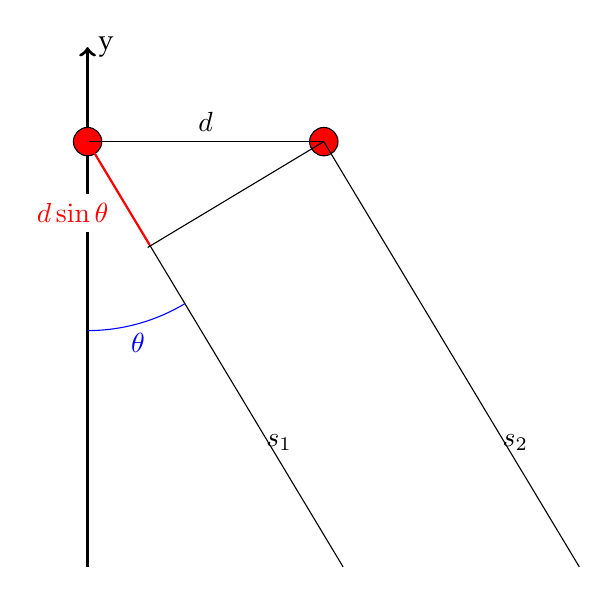
\begin{tikzpicture}[scale=3][>=stealth]

\def\thetanum{31}
\def\angle{59}
\def\ymax{2.0}
\def\xmax{3}
\def\yr{1.6}
\def\xv{1.2}
\def\d{1}
\def\sourcesize{0.06}
\def\arcsize{0.8}
	
% Colours
\colorlet{anglecolor}{blue} 
\colorlet{roadcolor}{gray!20!black} 
\colorlet{ycolor}{red} 
\colorlet{xcolor}{blue}
\colorlet{dcolor}{red}
	
% Styles  
\tikzstyle{important line}=[very thick] 
	
% Axes
\draw[important line, ->] (0, -0.2) -- (0, \ymax)  node[right]{y};
	
% Microphones
\filldraw[fill=ycolor, draw=black] (0, \yr) coordinate(M1) circle (\sourcesize);
\filldraw[fill=ycolor, draw=black] (\d, \yr) coordinate(M2) circle (\sourcesize);

\draw[-] (M1) -- ++(-\angle : 2.1) node[near end, above ]{$s_1$};
\draw[-] (M2) -- ++(-\angle : 2.1) node[near end, above ]{$s_2$};
\draw[- ] (M1) -- node[above] {$d$} (M2);
		
\draw[] (M2) -- ++(-90-\angle: \d*0.87) coordinate (dsin) ;
\draw[thick, dcolor] (M1) --  ++(-\angle : \d*0.51) node[anchor=north east, midway, fill=white]{$d \sin \theta$};

%\filldraw[fill=anglecolor!10!white, draw=anglecolor] (M1)  -- ++(0, -0.5)  arc(-90:-64.6:0.5) coordinate(ARC) -- cycle;
\draw[anglecolor] (M1)++(0, -\arcsize)  arc(-90:-\angle:\arcsize) coordinate(ARC) node[midway, below]{$\theta$};
	
\end{tikzpicture}


	\caption{Zoomed-in version of \Fig{overview} to show the difference in propagation distance $\Delta r=r_1-r_2$ from the sound source to the two  microphones. When the distance to the source is very long compared to the distance between the microphones, $r_1, r_2 \gg d$, the paths can be approximated as parallel and the difference is 
		$\Delta r\approx d sin \theta$. }
	\label{fig:far_field_zoom}
\end{stdfig}


\begin{enumerate}[a)]
	\item The delay from the sound is transmitted by the source to it is received by the microphone can be computed for both propagation paths. First, consider path $r_1$ from the vehicle to receiver M1. The time delay is the distance from the vehicle location at coordinate ($x_v$,0) to the
	receiver at coordinate (0,$y_r$), divided by the speed of sound $c$.
	The speed of sound in air can be set to $c$=\qty{340}{m/s}. 
	
	Write a mathematical expression for the time delay as function of the vehicle position $x_v$. 
	Call this delay $t_1$.
		
	\item Write a mathematical formula for the time delay of the signal that travels path $r_2$ from the transmitter at coordinate ($x_v$,0) to receiver M2 at coordinate ($d$, $y_r$).
	
	Call this delay $t_2$ and express it as a function of the vehicle position $x_v$.
	
	\item The signals at the two receivers, $x_1(t)$ at M1 and $x_2(t)$ at M2, are delayed copies of the transmitted signal,
	\begin{align*}
		x_1(t)&= s(t-t_1)  &	x_2(t)&= s(t-t_2)  
	\end{align*}
	where $s(t)$ is the transmitted sinusoidal signal.
	
	Assume that the source signal $s(t)$ is a zero-phase sinusoid at $f_0$=\qty{400}{Hz}, and set the amplitude of the transmitted signal to $A_s$=\num{1000}. 
	
	Make a plot of $x_1(t)$ and $x_2(t)$ when the vehicle is at position $x_v$=\qty{100}{m}.
	
	Plot 3 periods and measure the relative time-shift between the two received
	signals by comparing the peak locations.
	
	\item How do we convert relative time-shift into the direction $\theta$?
	
	The distance from the microphones to the source is often much larger than the distance between the microphones. We can then ignore that the angles from M1 and M2 are slightly different, and assume the paths to be close to parallel with the same angle $\theta$. This situation is illustrated in \Fig{far_field_zoom}, where we have zoomed in on the microphones in \Fig{overview}. 
	
	The difference $\Delta r$ in propagation distance for the two paths $r_1$ and $r_2$ from the source to the microphones can now be approximated to
	\begin{align}
		\Delta r = r_1-r_2 = d \sin\theta 
	\end{align}
	This is called the \emph{far field approximation} and is often used to find the beam pattern from antennas, loudspeakers, ultrasound trasnducers, and other sources.
	
	The propagation time $t$ along the paths is given as $t=r/c$, giving the time-shift $\Delta t$ between the signals arriving at the two microphones as
	\begin{align}
		\Delta t = t_1-t_2 = \frac{d \sin\theta }{c} \:,
	\end{align}
	which corresponds to a phase-shift $\Delta \phi$ between the two signal of
	\begin{align}
		\Delta \phi = -2\pi \Delta t f_s = -2 \pi \frac{d f_s \sin\theta }{c} 
		= -2 \pi \frac{d \sin\theta }{\lambda_s}\:,
		\label{eq:phaseshift-approximated}
	\end{align}
	where $\lambda_s=c/f_s$ is the wavelength of the emitted sound.
	
	Calculate $\theta$ for the time-shift you found in the example above.
	
	In addition, use geometry and the values of $x_v$ and $y_r$ to find the true value of $\theta$, i.e., not using the approximation \Eq{phaseshift-approximated}. 
	
	Compare the two results and compare your calculated value of $\theta$ to the true value.
	
	\item The objective in the rest of this lab is to write a Python function that will process the received signals to find the direction $\theta$. 
	
	Calculate the complex amplitudes $X_1 = A_1 e^{j\phi_1}$ and $X_2 = A_2 e^{j\phi_2}$ received at M1 and M2 as function of vehicle position $x_v$
	
	Show that you can compute the phase difference between two phasors $X_1$ and $X_2$ by the equation
	\begin{align*}
		\Delta \phi = \angle \{ X_1 X_2^* \}
	\end{align*}
	where the superscript * denotes the complex conjugate. Use the ideas presented here, summarised in \Fig{far_field_zoom} and \Eq{phaseshift-approximated}, to write a Python-function that will compute the direction $\theta$ from the complex amplitudes.
		
	\item Run your function for the vehicle moving from $x_v$=\qty{-400}{m} meters to  $x_v$=\qty{+500}{m} in steps of one meter.
	
	Compare the value of $\theta$ calculated from the phase difference to the true value of $\theta$ by plotting both on the same graph.
	
	Comment the result.
		
\end{enumerate}

\bibliographystyle{ieeetr}
\bibliography{../defs/tse2280.bib}
\end{document}